\chapter{Mechanical Design}

\graphicspath{{./Figures/Mechanical Design/}}
%	\item Outline the purpose and scope of the chapter.
 Modeling In this chapter, the details of the mechanical design are presented.
 where it goes from the initial conceptual design to the final design showing in the process the design decision-making for each critical point, This chapter emphasis the detailed description of the precise placement and alignment of different components such as the motors, wheels, battery, boards, and others to maintain the seamless integration of all the components into the robot body.
%	\item Briefly describe the mechanical design's role in the overall project.
\newline
The mechanical design serves as an important pillar to define the new physical form, size, and shape of the TWIPR. Depending on how these criteria are defined, the robot would interact with the environment.
taking into account that the design directly influences the center of gravity, which is crucial to consider in our robot due to the inverted pendulum nature to be able to balance and maintain the upright position.
In addition to the impact that the design has on the maneuverability of the robot and how it would respond to the control signals to be able to execute a task.
\newpage
\section{Design Objectives and Requirements}

%	Detail the primary objectives of the mechanical design
	The main objective is to come up with a new design for a multiple joints Robot to perform complex dynamic movements.
	This robot would be based on the Two wheeled inverted pendulum robots.
	The new design would add more degrees of freedom to enable the more complex movements.
	This enhances the robot's capabilities where it can execute more diverse scenarios.
%	\item List the requirements that the design must meet (e.g., weight limits, size constraints, mobility requirements).
	Initially, the main requirement was to add two more degrees of freedom where originally it used to have one degree of freedom in the wheels.
	The new design has three degrees of freedom, one in the wheels, one as a knee joint and one as a hip joint.
	The current design has two identical legs.

\section{Conceptual Design}
%Discuss the initial design concepts.
As for the initial design concepts the body was that main point of focus as shown in the figure \ref{fig:initialdesigns}.Three initial designs where considered mainly for the body.\ Symmetrical vertical body in figure A, symmetrical horizontal body in figure B and leaning forward body in figure C\@.
\ For the three designs, two independent legs where considered.
two designs where considered for the legs, the normal joint leg and the compliant leg

\begin{figure}[h]
	\centering
	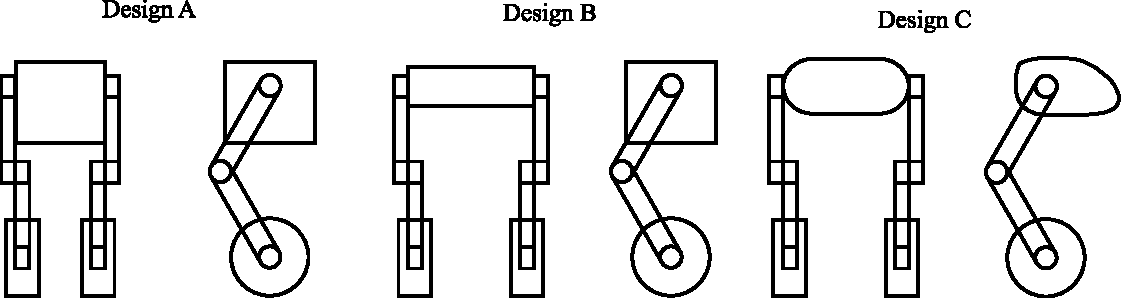
\includegraphics[width=1\linewidth]{Conceptual Design}
	%\includegraphics[width=0.5\linewidth]{Figures/Mechanical Design/Conceptual_Design}
	\caption[Initial Design Concepts]{Three Initial Design Concepts for the robot}
	\label{fig:initialdesigns}
\end{figure}
Two main designs where considered for the legs as shown in the figure \ref{fig:legdesignsjbhi}, the normal joint leg and the compliant leg.
The compliant leg is more flexible and can be used to absorb the shock from the ground.\ The normal joint leg is more rigid and can be used to generate more torque.in addition, the normal is more relative to our use-case as it can precisely control the position of the leg.
% figure for the leg designs concepts
\begin{figure}[h]
	\centering
	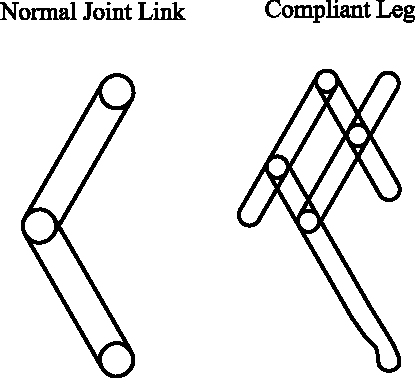
\includegraphics[width=0.4\linewidth]{Leg Design}
	\caption[Leg Design Concepts]{Leg Design Concepts}
	\label{fig:legdesignsjbhi}
\end{figure}

%Explain the decision-making process for selecting the final concept.
% Include sketches or early design models.
\section{Schmatic Representation of the Robot}
% the schematic representation of the robot should show the location of the different components such as the motors, wheels, battery, boards, and others
%figure for the schematic representation of the robot
\subsection{Schmatic overview of the robot}
%figure for the schmatic overview of the robot
\begin{figure}[h]
	\centering
	\includegraphics[width=0.5\linewidth]{Schmatic Overview of the robot}
	\caption[schmatic overview of the robot]{schmatic overview of the robot}
	\label{fig:schmaticoverviewoftherobot}
\end{figure}
As shown in the figure \ref{fig:schmaticoverviewoftherobot}, In order to achieve the desired movements using the new articulated legs, then we need three motors on each leg, one motor for the wheel, one motor for the knee joint and one motor for the hip joint.
In addition to the motors, the robot needs a battery to power the motors, a control board to control the motors, and a power management board to manage the power distribution between the different components. Some of the components  are passed on from the previous TWIPR robot such as the control board, the power management board. For more information about the electronic components and there specifications, please refer to the electronics design chapter.

\section{Initial Calculations}
%figure for the initial calculations
\begin{figure}[h]
	\centering
	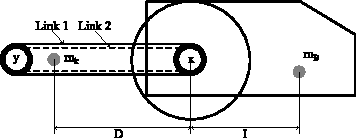
\includegraphics[width=0.7\linewidth]{Initial Calculations}
	\caption[Initial Calculations]{Initial Calculations}
	\label{fig:initialcalculations}
\end{figure}
One of the main critical positions for the robot, as shown in the figure \ref{fig:initialcalculations} is the position where the center of mass of the body and the center of mass of the legs are the furthest away from point x on the horizontal axis.It is important to make the initial torque calculations to be able to select the right motors for the robot.
Starting from that position first, the robot should be able to balance itself and maintain the upright position.
secondly, the robot should be able to change the knee angle to lift the body while maintaining its balance.
The calculations are based on some assumptions and simplifications, Considering only half the body weight and one leg.
As shown in the figure, The Wheel motor shaft is aligned with the hip joint, the minimum torque required to balance the robot is calculated as follows:

The summation of the torques around point x should be equal to zero to maintain the balance with minimum motor torque.
\begin{equation}
	\sum_{i=1}^{n} \tau_{i}=0
\end{equation}
\begin{equation}
	\sum_{i=1}^{n} \tau_{i}=m_{\mathrm{B}}gI-m_{\mathrm{K}}g(0.7)D
\end{equation}
\begin{equation}
	\sum_{i=1}^{n} \tau_{i}=0.704(9.81)(0.03)-0.2(9.81)(0.7)(0.15)\approx0\,\mathrm{Nm}
\end{equation}
The Lengths of D and I can be modified to make sure that the summation of the torques around point x is equal or approximately equal to zero.
This will make sure that the robot can balance itself with minimum wheel motor torque.
The torques can cancel each other out by readjusting the lengths of D or I and also by modeling the weight distribution in the body and the legs.

The torque required to lift the body is calculated around the knee joint point y as follows:
\begin{equation}
	\sum_{i=1}^{n} \tau_{i}=m_{\mathrm{B}}g(D+I)-m_{\mathrm{K}}g(0.3)D
\end{equation}
\begin{equation}
	\sum_{i=1}^{n} \tau_{i}=0.704(9.81)(0.03+0.15)-0.2(9.81)(0.3)(0.15) \approx 1.154 \,\mathrm{Nm}
\end{equation}
1.154 $\mathrm{Nm}$ is the minimum torque required to hold the body in position.
The Knee motor should be able to generate more torque to be able to lift the body and change the knee angle.

The approximate masses of the body and the legs are estimated in the table\ref{tab:initialcalculationsassumptions}.
After manufacturing the parts and assembling the robot, the actual masses of the body and the legs are measured and the calculations are updated accordingly.
\begin{table}[h]
    \centering
    \caption{Initial Calculations Assumptions}
    \label{tab:initialcalculationsassumptions}
    \begin{tabular}{lcl}
        \toprule
        Parameter & Value & Description \\
        \midrule
        $m_{\mathrm{B}}$         & 0.704\,kg  & Mass of the body \\
        $m_{\mathrm{K}}$         & 0.2\,kg    & Mass of the Knee including the two legs \\
        $L_1$                    & 0.15\,m    & Length of Link 1 \\
        $L_2$                    & 0.15\,m    & Length of Link 2 \\
        $D$                      & 0.03\,m    & Distance from the Wheel axis to the center of mass of leg \\
        $I$                      & 0.03\,m    & Distance from the hip joint axis to the center of mass of the body \\
        \bottomrule
    \end{tabular}
\end{table}

\begin{notebox}
	\textbf{To reduce the needed torque to lift we can:}
	%bullit points
	\begin{itemize}
		\item Shorten the links
		\item Reduce the body weight
		\item Use gearbox to increase the torque
	\end{itemize}
\end{notebox}
%To reduce the needed torque to lift the body, we can:
%\begin{itemize}
%	\item Shorten the links
%	\item Reduce the body weight
%	\item Use gearbox to increase the torque
%\end{itemize}

\newpage
\section{Detailed Design Development}
% Elaborate on the development of the detailed mechanical design.
Throughout the design process, modularity and ease of assembly were considered.
The design was broken down into three main parts: the body, the hip-knee link, and the knee-wheel link.
Print iterations were made to ensure that the parts fit together and that the robot could be assembled with ease.
Modifications were made to simplify the printing process and reduce the support material used.
Detailed technical drawing figures with dimensions for the fully assembled robot are shown at the end of the chapter in \ref{fig:robotassemblyv2side} \ref{fig:robotassemblyv2top}.


\subsection{Body Design}
% Discuss the design of the body.
The body design is the main part of the robot, it is the main structure that holds all the components together.
The components that are mounted on the body are the hip motors, the battery, camera, sensor, a rack that includes the power distribution board, the microcontroller board attached to the Raspberry Pi. The optimization of the body design is crucial to be able to fit all the components in a compact form and at the same time distribute the weight equally to maintain the balance of the robot.
Different design features were considered, such as the cable management, the fastening features specifically designed to easily mount the battery, organizing the cable between the boards and the rest of the robot parts.
Opening slots were to one side of the body to be able to access the boards and connect charging cables to the battery.
%figure 1 for the body design
\begin{figure}[h]
	\centering
	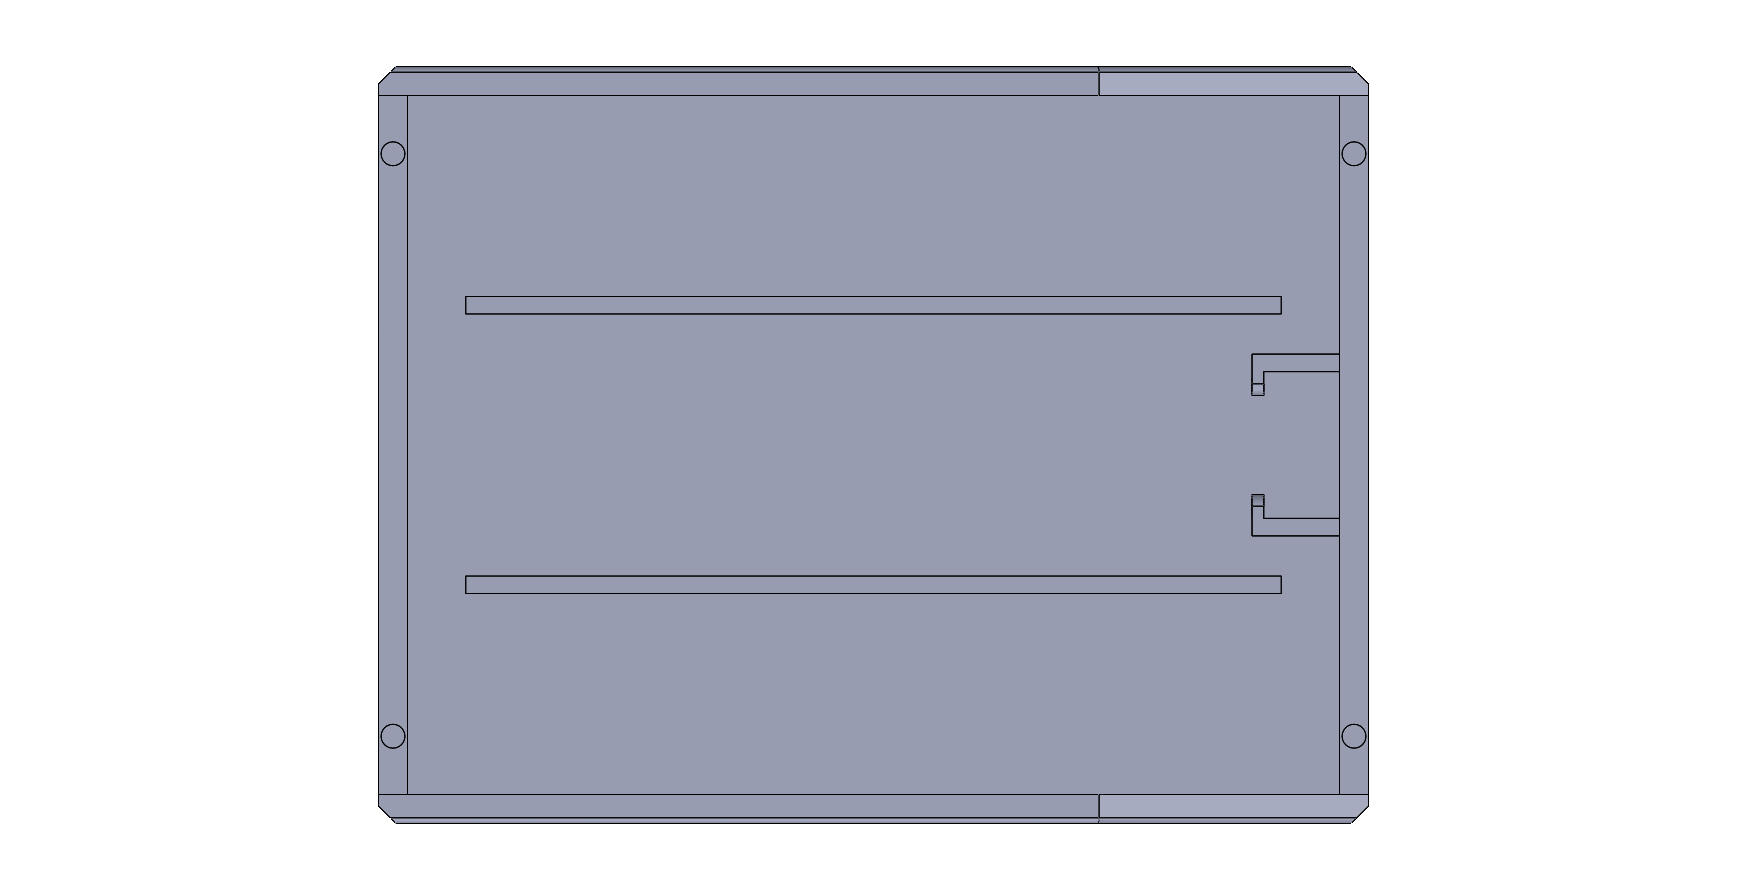
\includegraphics[width=1\linewidth]{Body_Design_1}
	\caption[Top view of the Body Design]{Top view of the Body Design}
	\label{fig:bodydesign1}
\end{figure}
%figure 2 for the body design
\begin{figure}[h]
	\centering
	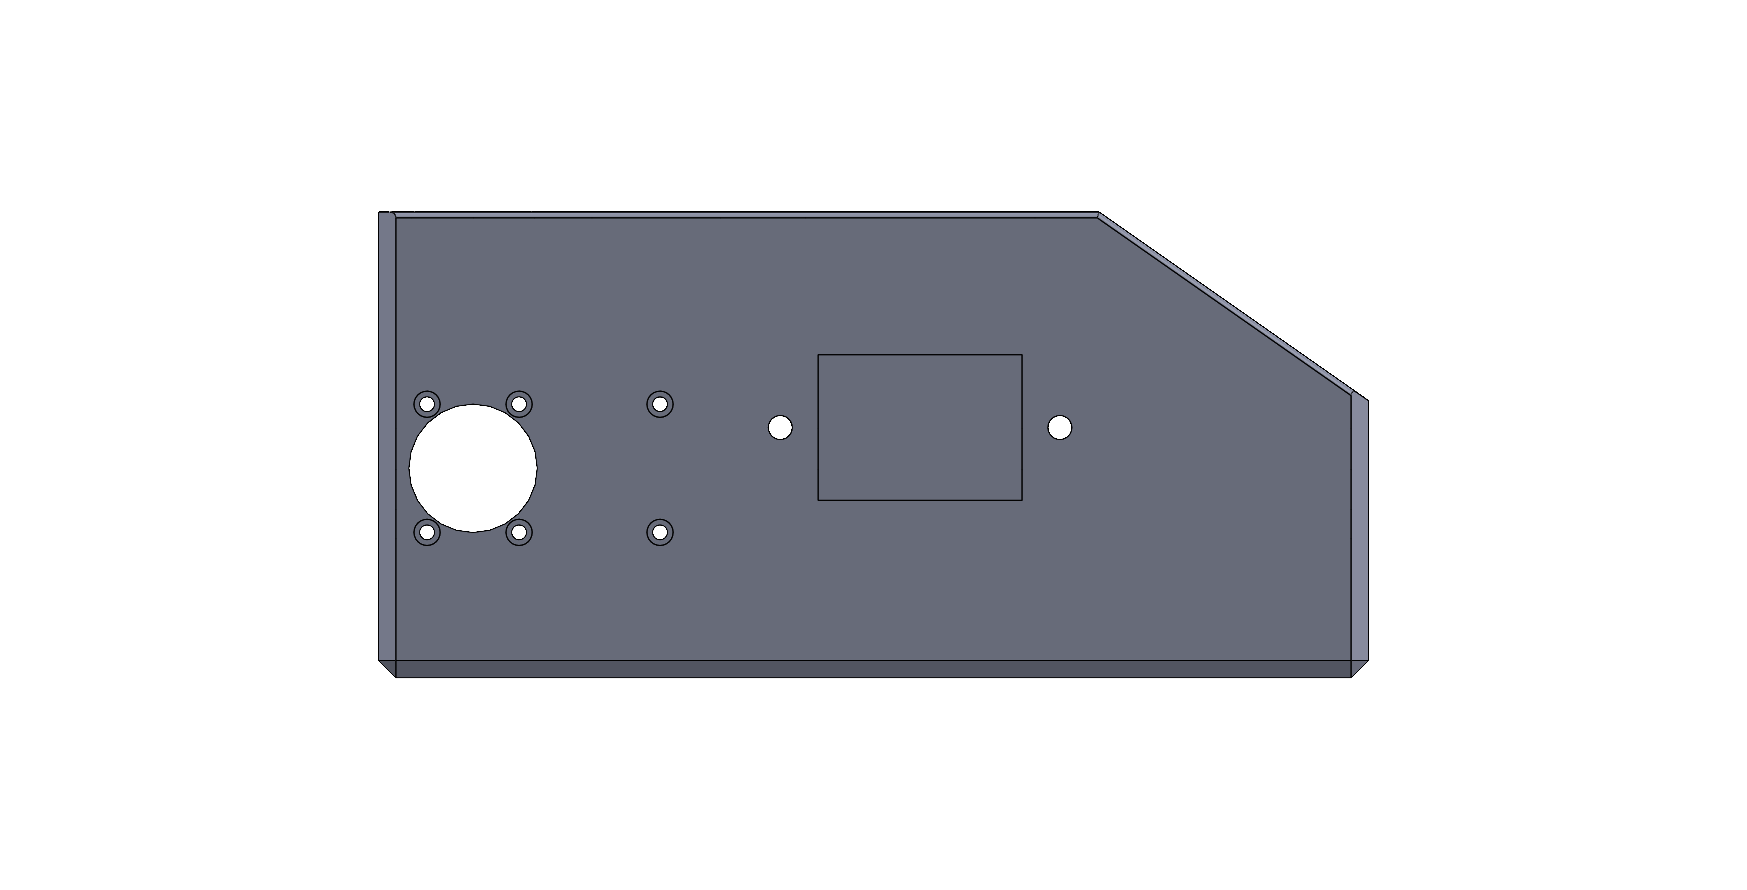
\includegraphics[width=1\linewidth]{Body_Design_2}
	\caption[Side view of the Body Design]{Side view of the Body Design}
	\label{fig:bodydesign2}
\end{figure}
\vspace{10cm}
%figure 3 for the body design
\begin{figure}[h]
	\centering
	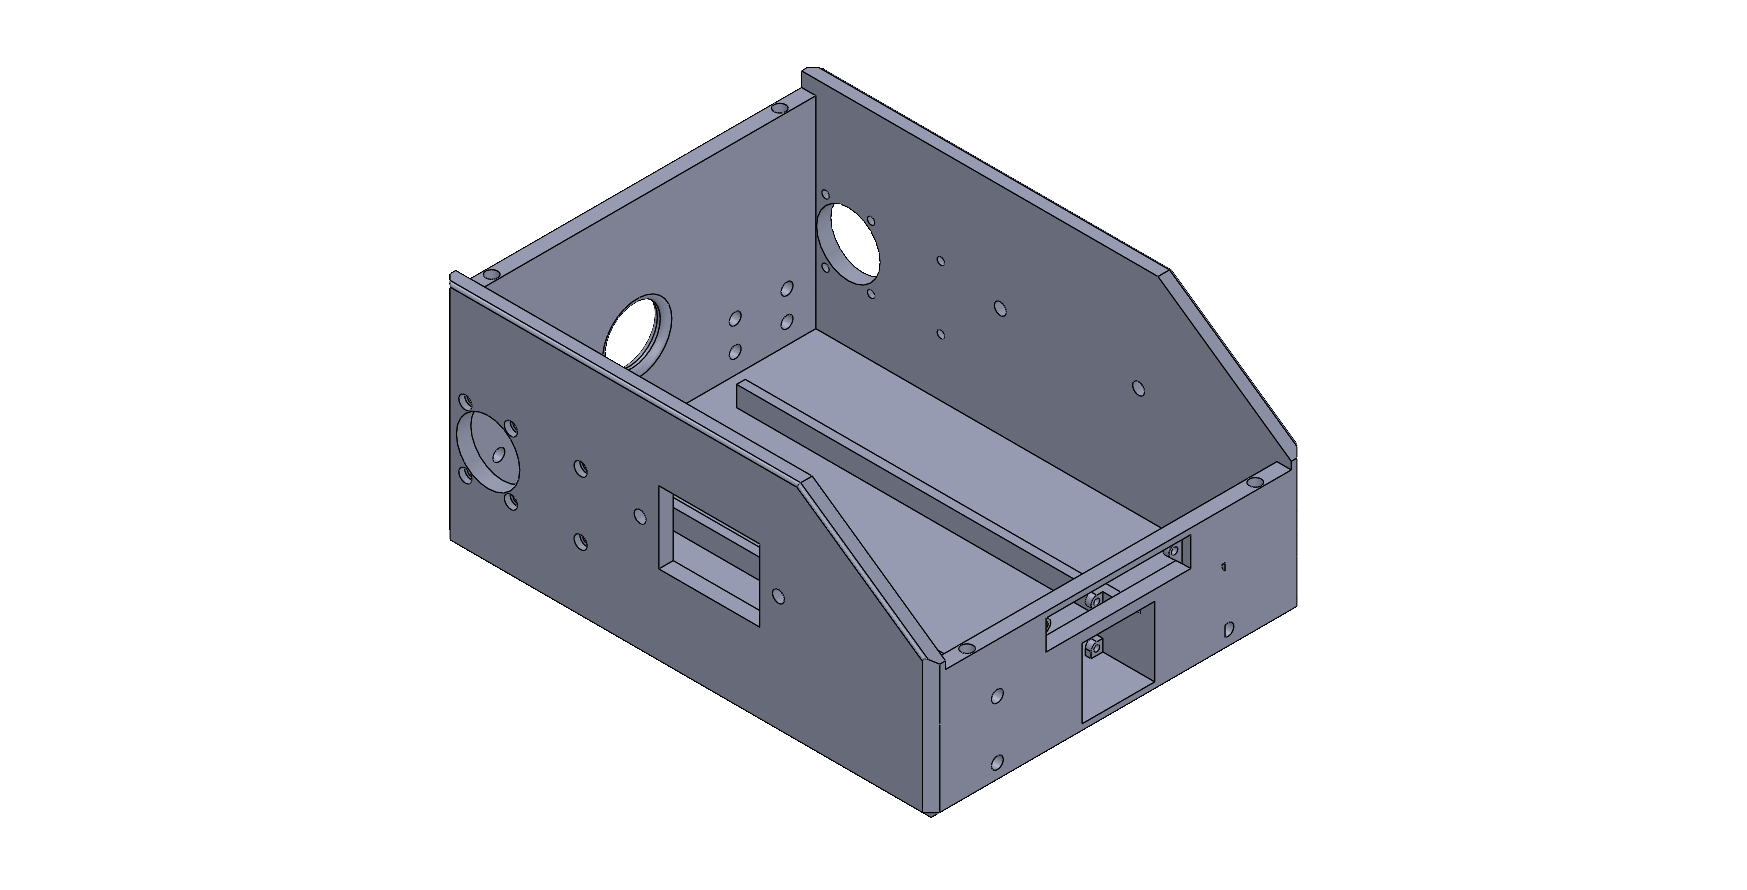
\includegraphics[width=0.8\linewidth]{Body_Design_3}
	\caption[3D view of the Body Design]{3D view of the Body Design}
	\label{fig:bodydesign3}
\end{figure}

\newpage
\subsection{Hip Knee Link Design}
% Discuss the design of the hip knee Link.
This link connects the hip body axis to the knee axis.
The design of this link includes the knee motor housing form one-side and a frame to attach to the output horn of the hip motor.
The motor housing is designed to ensure the fixed placement of the motor inside the link, As shown in the figure, \ref{fig:bodykneelink1} Cable management is also considered in the design of this link to make sure that the cables are not interfering with the movement of the link.The curvature of the link creates enough clearance so that when the hip axis is aligned with the wheel axis, they would not touch with each other even when considering the elastic bending of the legs.
%figure 1 for the Body_Knee_link
\begin{figure}[h]
	\centering
	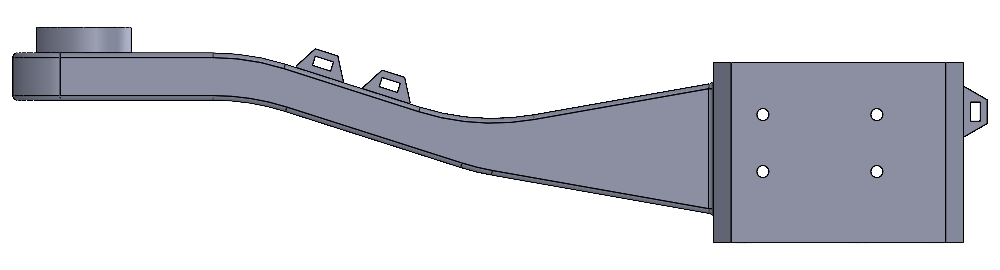
\includegraphics[width=1\linewidth]{Body_Knee_Link_1}
	\caption[Top view of the Body Knee Link]{Top view of the Body Knee Link}
	\label{fig:bodykneelink1}
\end{figure}
%figure 2 for the Body_Knee_link
\begin{figure}[h]
	\centering
	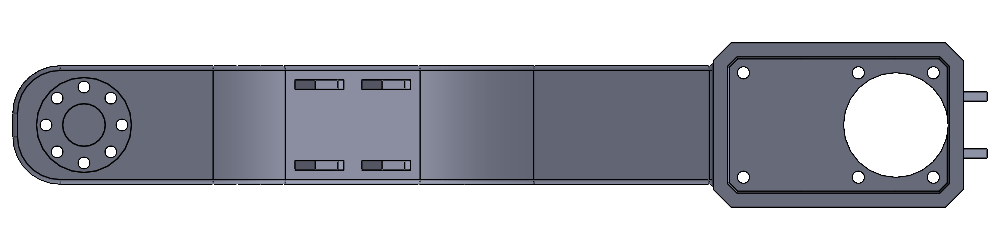
\includegraphics[width=1\linewidth]{Body_Knee_Link_2}
	\caption[Side view of the Body Knee Link]{Side view of the Body Knee Link}
	\label{fig:bodykneelink2}
\end{figure}
%figure 3 for the Body_Knee_link
\begin{figure}[h]
	\centering
	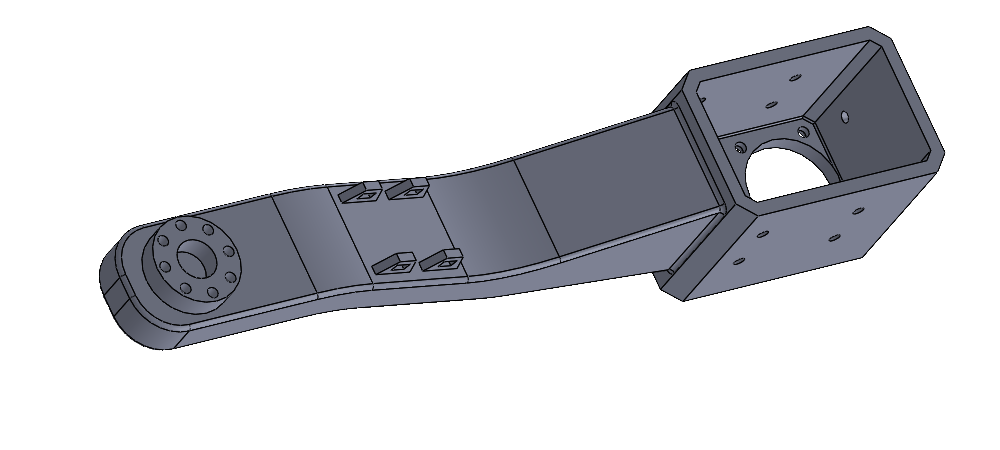
\includegraphics[width=1\linewidth]{Body_Knee_Link_3}
	\caption[3D view of the Body Knee Link]{3D view of the Body Knee Link}
	\label{fig:bodykneelink3}
\end{figure}

\newpage
\subsection{Knee Wheel Link Design}
% Discuss the design of the Wheel_Knee_link.
This link connects the knee axis to the wheel axis.
The design of this link includes the wheel motor mounting form one-side and a frame to attach to the output horn of the knee motor from the other side. The motor mounting is designed to ensure the fixed placement of the motor on the link, As shown in the figure, \ref{fig:wheelkneelink2}. Cable management is also considered in the design of this link by adding a cable fastener and holes to pass the cables through the link.
%figure 1 for the Wheel_Knee_link
\begin{figure}[h]
	\centering
	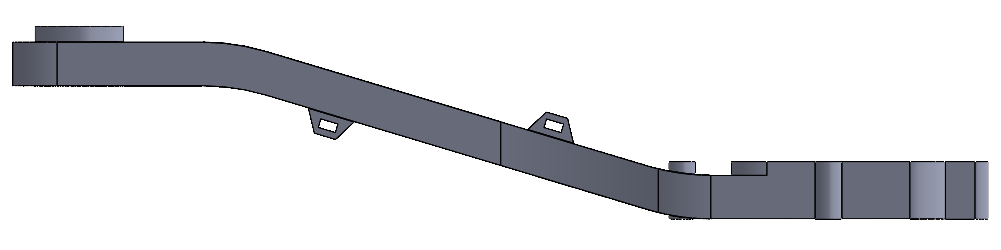
\includegraphics[width=1\linewidth]{Wheel_Knee_Link_1}
	\caption[Side view of the Knee Wheel Link]{Side view of the Knee Wheel Link}
	\label{fig:wheelkneelink1}
\end{figure}
%figure 2 for the Wheel_Knee_link
\begin{figure}[h]
	\centering
	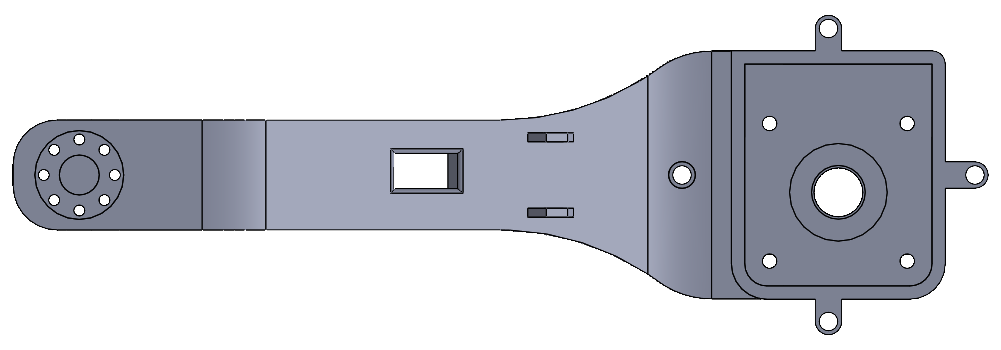
\includegraphics[width=1\linewidth]{Wheel_Knee_Link_2}
	\caption[Top view of the Knee Wheel Link]{Top view of the Knee Wheel Link}
	\label{fig:wheelkneelink2}
\end{figure}
%figure 3 for the Wheel_Knee_link
\begin{figure}[h]
	\centering
	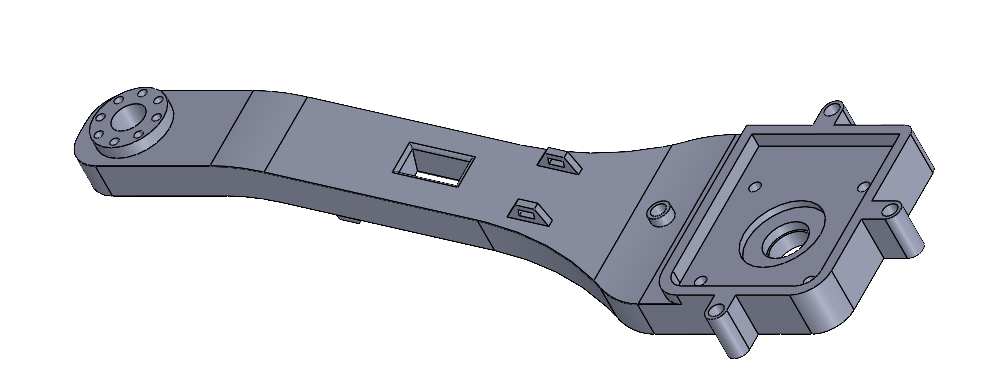
\includegraphics[width=1\linewidth]{Wheel_Knee_Link_3}
	\caption[3D view of the Knee Wheel Link]{3D view of the Knee Wheel Link}
	\label{fig:wheelkneelink3}
\end{figure}


\newpage
\subsection{Boards Mounting rack}
% Discuss the design of the Boards Mounting rack.
As shown in the figure \ref{fig:pcbrack1},\ref{fig:pcbrack2},\ref{fig:pcbrack3}, the board mounting rack is designed to hold the power distribution board, the microcontroller board, and the Raspberry Pi.
The rack is designed to be mounted in the body of the robot by using four screws.
Appropriate space is considered between the two boards as well as the clearance between the rack and the battery underneath it and the body cover on top of it.
%figure 1 for the PCB_Rack
\begin{figure}[h]
	\centering
	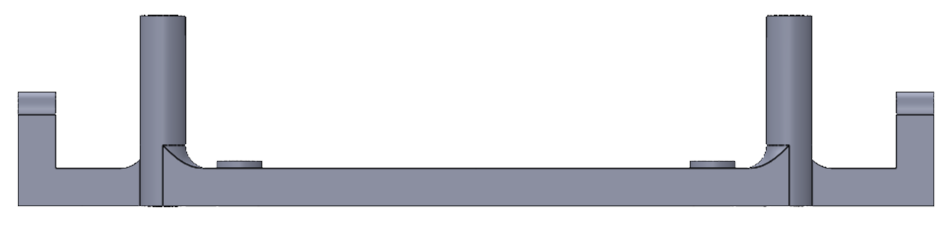
\includegraphics[width=.7\linewidth]{PCB_Rack_1}
	\caption[Side view of the PCB Rack]{Side view of the PCB Rack}
	\label{fig:pcbrack1}
\end{figure}
%figure 2 for the PCB_Rack
\begin{figure}[h]
	\centering
	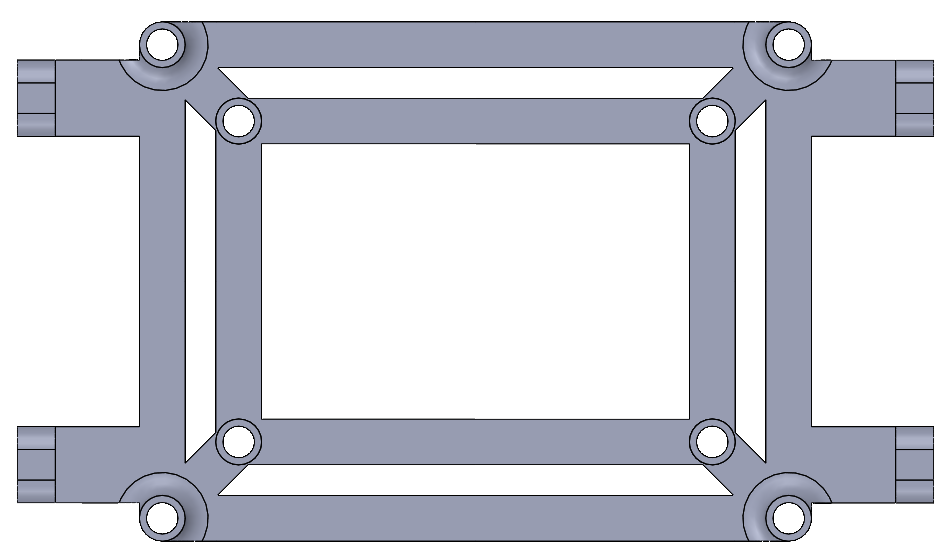
\includegraphics[width=.7\linewidth]{PCB_Rack_2}
	\caption[Top view of the PCB Rack]{Top view of the PCB Rack}
	\label{fig:pcbrack2}
\end{figure}
%figure 3 for the PCB_Rack
\begin{figure}[h]
	\centering
	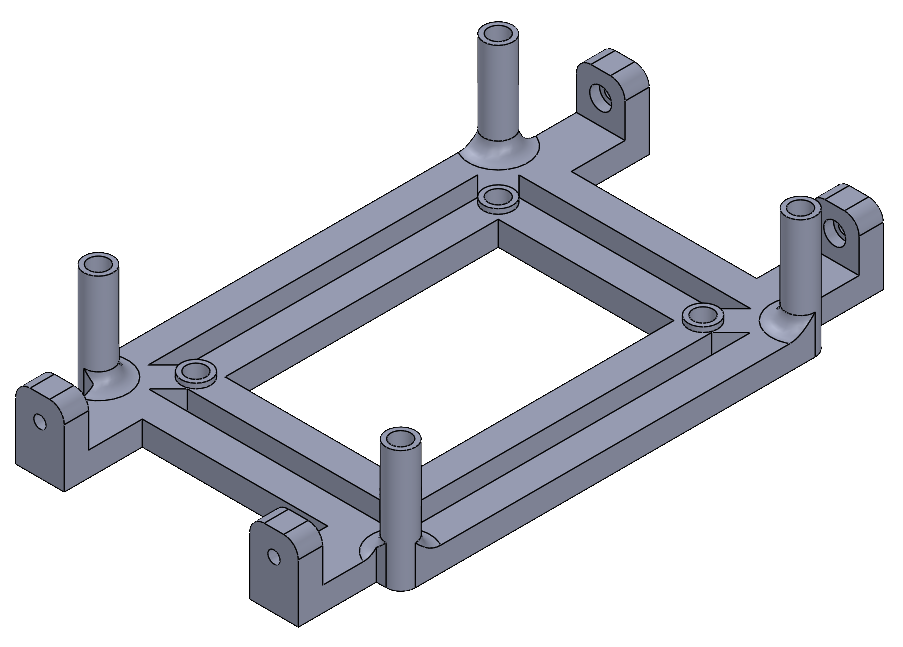
\includegraphics[width=.7\linewidth]{PCB_Rack_3}
	\caption[3D view of the PCB Rack]{3D view of the PCB Rack}
	\label{fig:pcbrack3}
\end{figure}
\newpage
\subsection{Motor Cover}
% Discuss the design of the Motor Cover.
The motor cover is designed to protect the motor from any external objects that might interfere with the motor operation.
The motor cover is designed to be mounted on the wheel knee link with the consideration of the clearance between the motor cover and hip knee link.
Slots are designed to dissipate the heat generated from the motor as shown in the figure \ref{fig:motorcover1}, \ref{fig:motorcover3}.
%fugure 1 for the motor_cover
\begin{figure}[h]
	\centering
	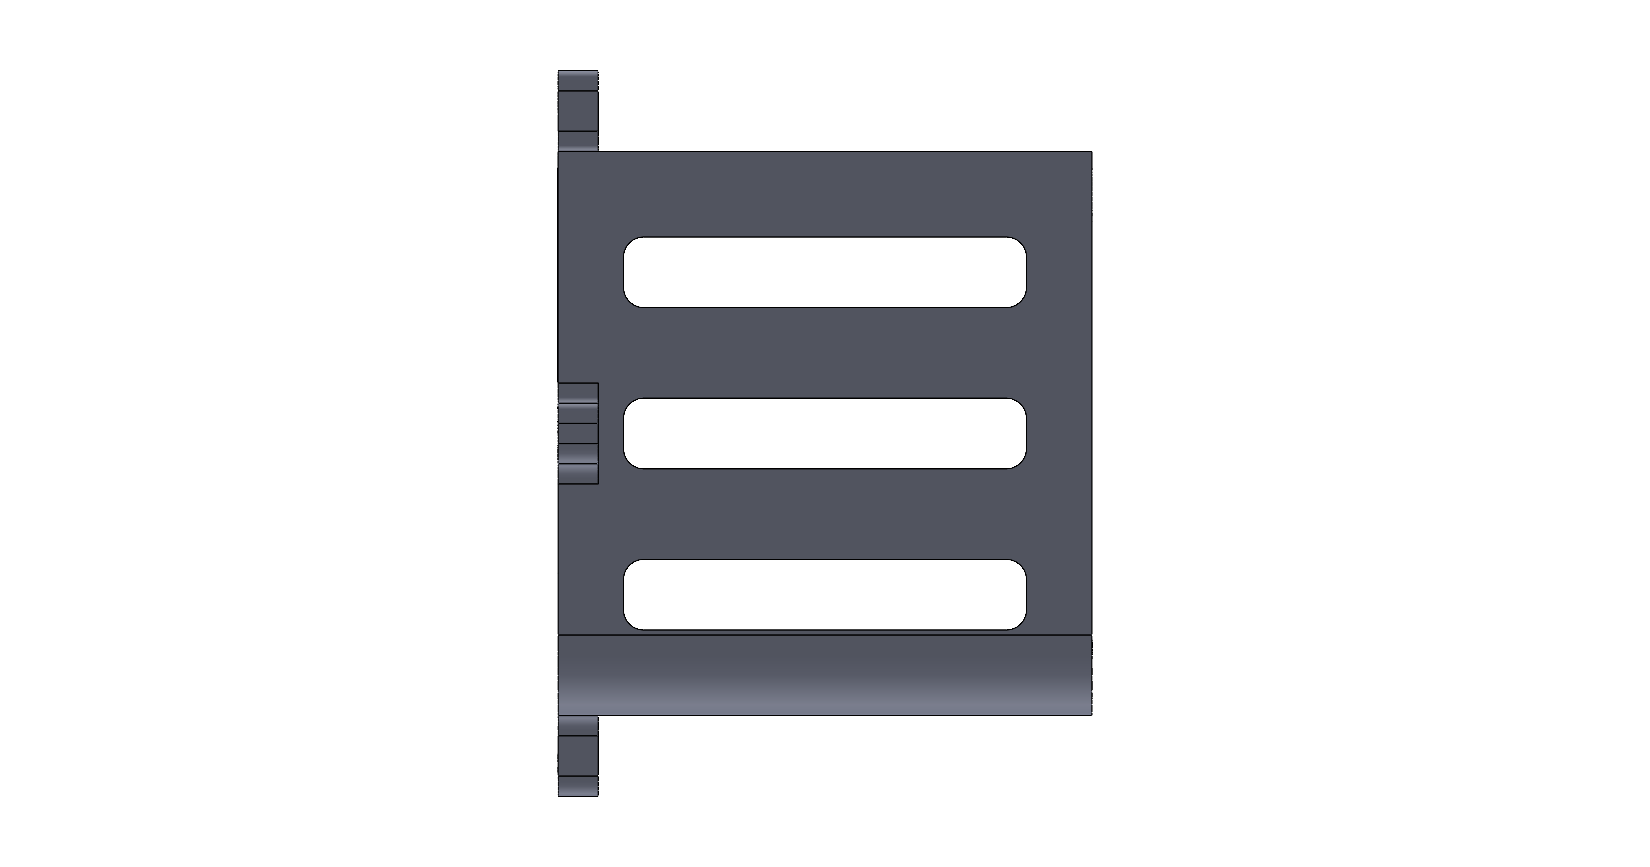
\includegraphics[width=.6\linewidth]{motor_cover_1}
	\caption[Side view of the Motor Cover]{Side view of the Motor Cover}
	\label{fig:motorcover1}
\end{figure}
%fugure 2 for the motor_cover
\begin{figure}[h]
	\centering
	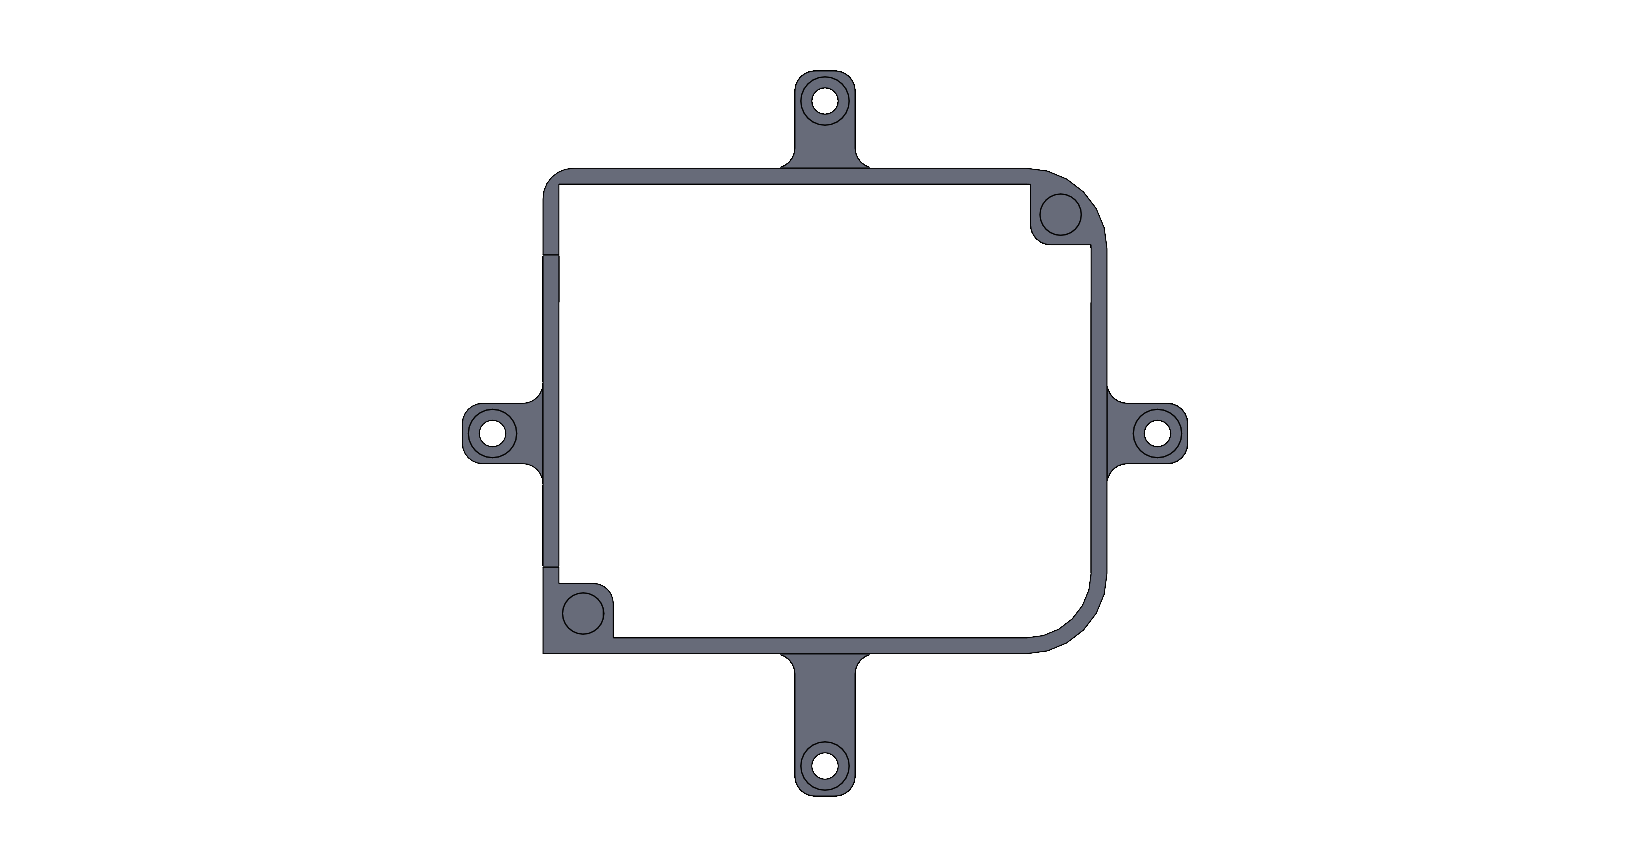
\includegraphics[width=.6\linewidth]{motor_cover_2}
	\caption[Top view of the Motor Cover]{Top view of the Motor Cover}
	\label{fig:motorcover2}
\end{figure}
%fugure 3 for the motor_cover
\begin{figure}[h]
	\centering
	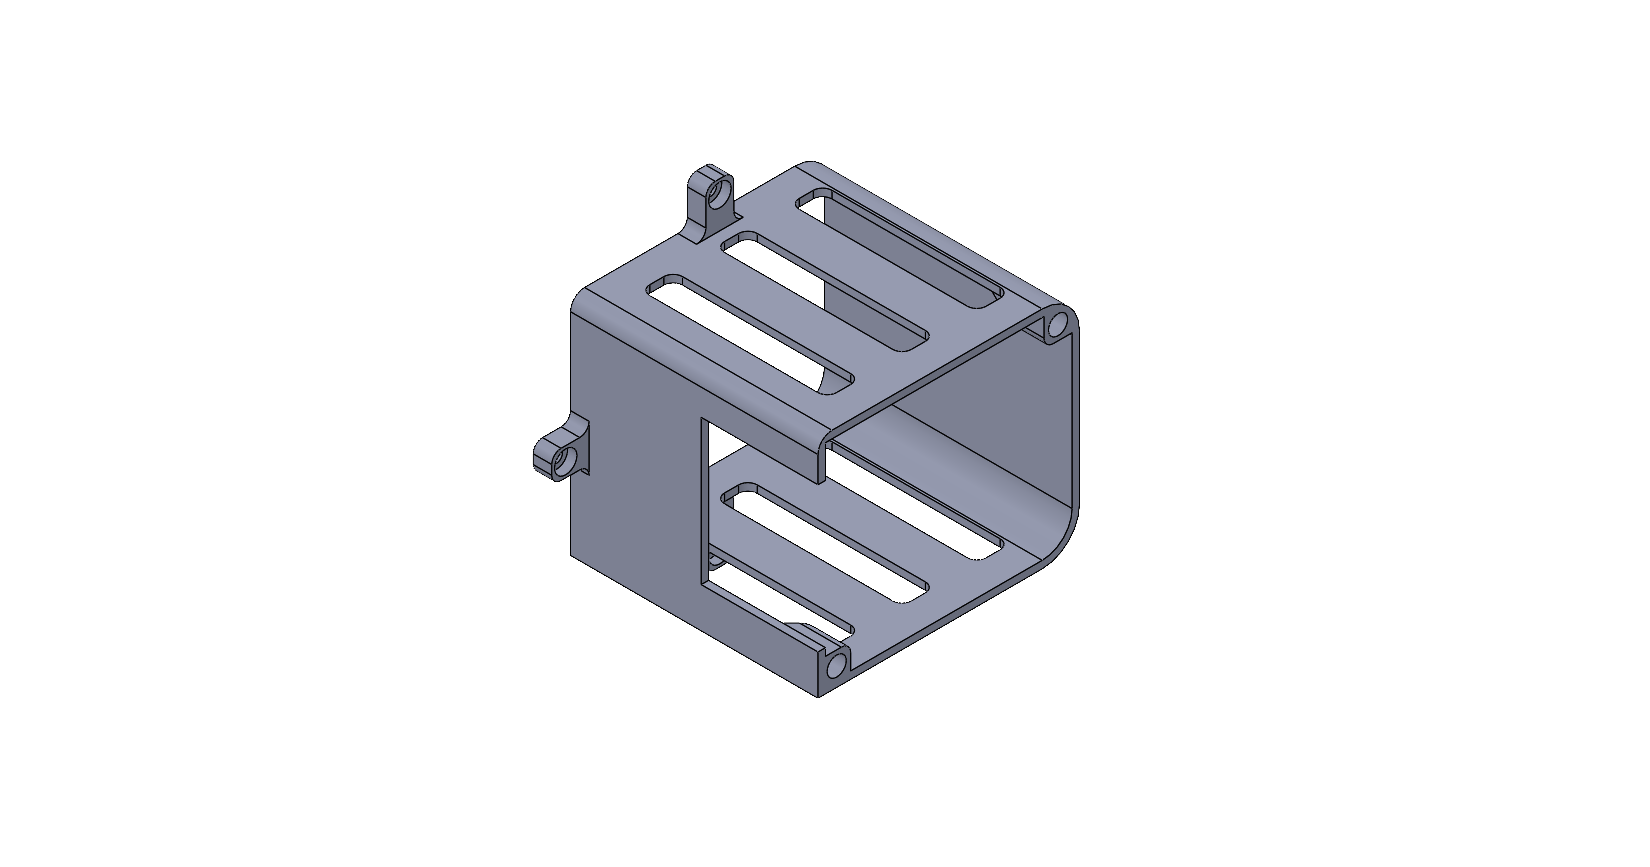
\includegraphics[width=.6\linewidth]{motor_cover_3}
	\caption[3D view of the Motor Cover]{3D view of the Motor Cover}
	\label{fig:motorcover3}
\end{figure}


\newpage
\subsection{Full Design}


%figure 1 for the Robot_Assembly
\begin{figure}[h]
	\centering
	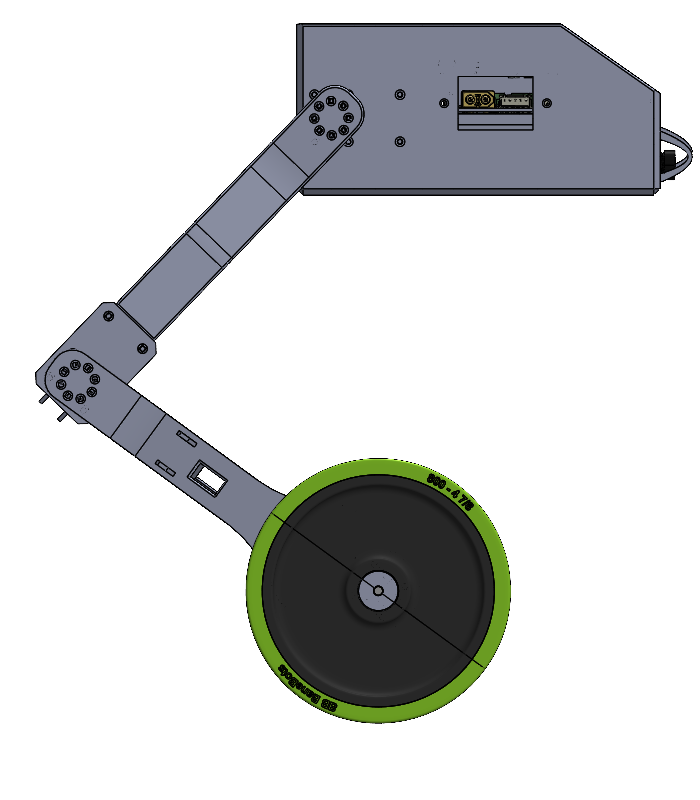
\includegraphics[width=.6\linewidth]{Robot_Assembly_1}
	\caption[Side view of the Robot Assembly]{Side view of the Robot Assembly}
	\label{fig:robotassembly1}
\end{figure}
%figure 2 for the Robot_Assembly
\begin{figure}[h]
	\centering
	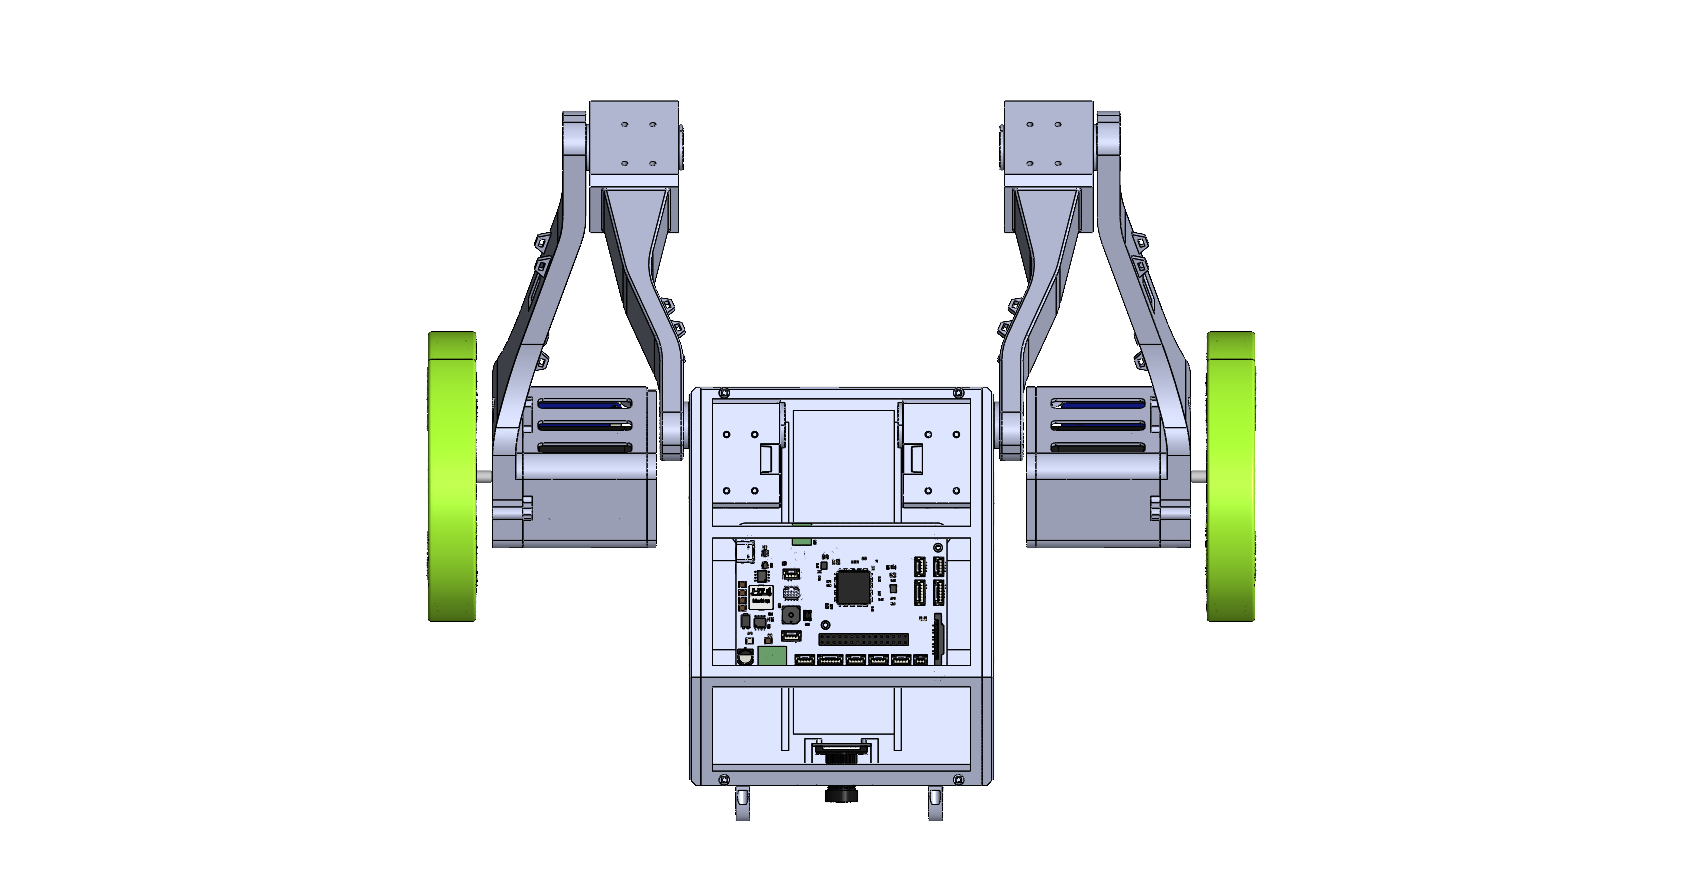
\includegraphics[width=.6\linewidth]{Robot_Assembly_2}
	\caption[Top view of the Robot Assembly]{Top view of the Robot Assembly}
	\label{fig:robotassembly2}
\end{figure}
%figure 3 for the Robot_Assembly
\begin{figure}[h]
	\centering
	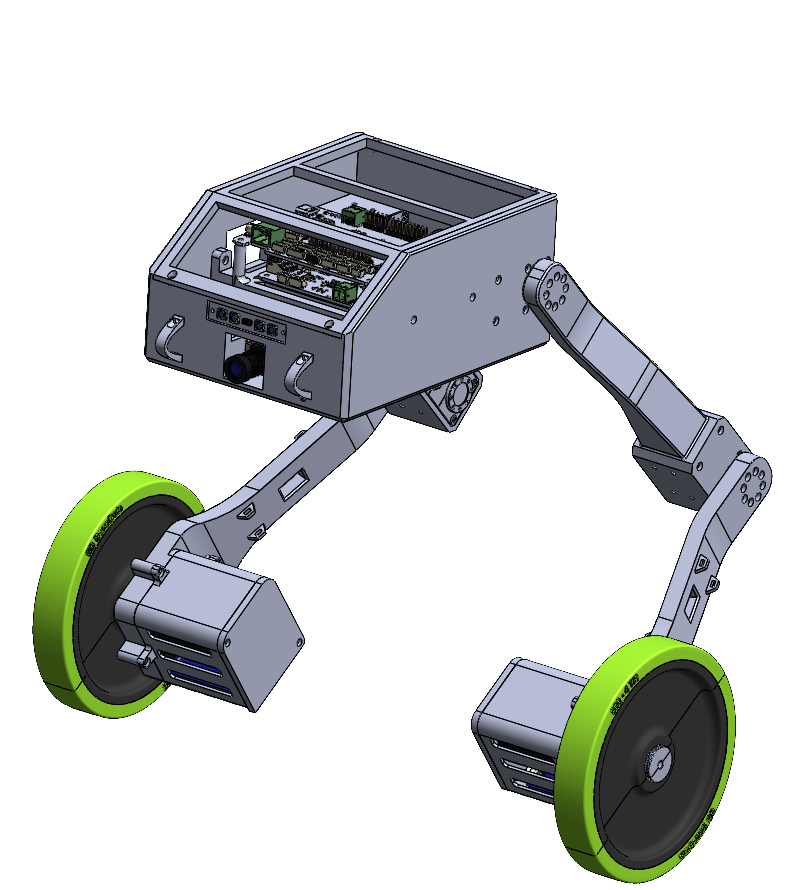
\includegraphics[width=1\linewidth]{Robot_Assembly_3}
	\caption[3D view of the Robot Assembly]{3D view of the Robot Assembly}
	\label{fig:robotassembly3}
\end{figure}
\vspace{3cm}
The full design of the robot is shown in the figure\ref{fig:robotassembly3}.
The robot is designed to be assembled in a modular way.
The full assembly reveals how all the parts fit together.
This includes the body, the hip-knees, the knee-wheel links, the motor cover, the boards mounting rack,the hip motors, the knee motors, the camera, the sensor, the face shield, the body cover,the BaneBots shaft hub, and the wheels.
After assembling the robot, different movements configurations are tested using the CAD software to make sure that the robot can move freely without any interference between the different parts.
\newpage
%sub section for the dimentions of the robot
\subsection{Dimensions}
%figure for the dimensions of the robot
As shown in the figure \ref{fig:robotassemblyv2side}, \ref{fig:robotassemblyv2top}, the main dimensions of the robot are shown.
Comparing the dimensions of the robot to the dimensions of the previous TWIPR robot, the new robot is much bigger in size because of the addition of the two legs.
Compactness was not a main concern in the design of the robot, the main concern was to make sure that the robot can perform the required movements and interact with the environment.
\begin{figure}[h]
	\centering
	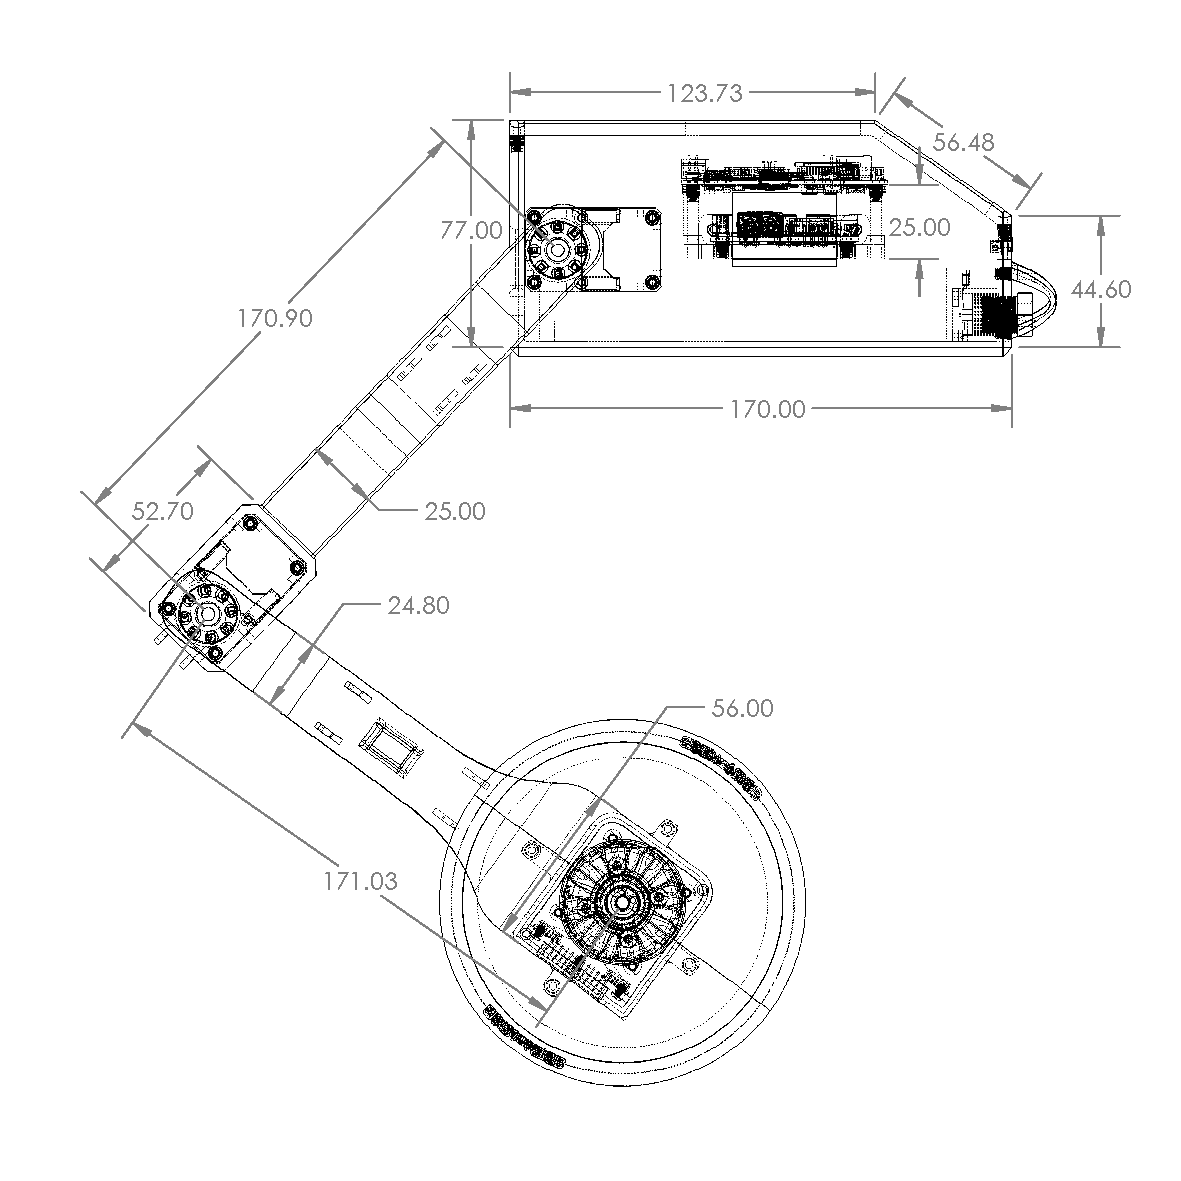
\includegraphics[width=\linewidth]{Robot_Assembly_V2_Side}
	\caption[Side view of the Robot Assembly]{Side view of the Robot Assembly}
	\label{fig:robotassemblyv2side}
\end{figure}
\vspace{4cm}
%figure for the dimensions of the robot top view
\begin{figure}[h]
	\centering
	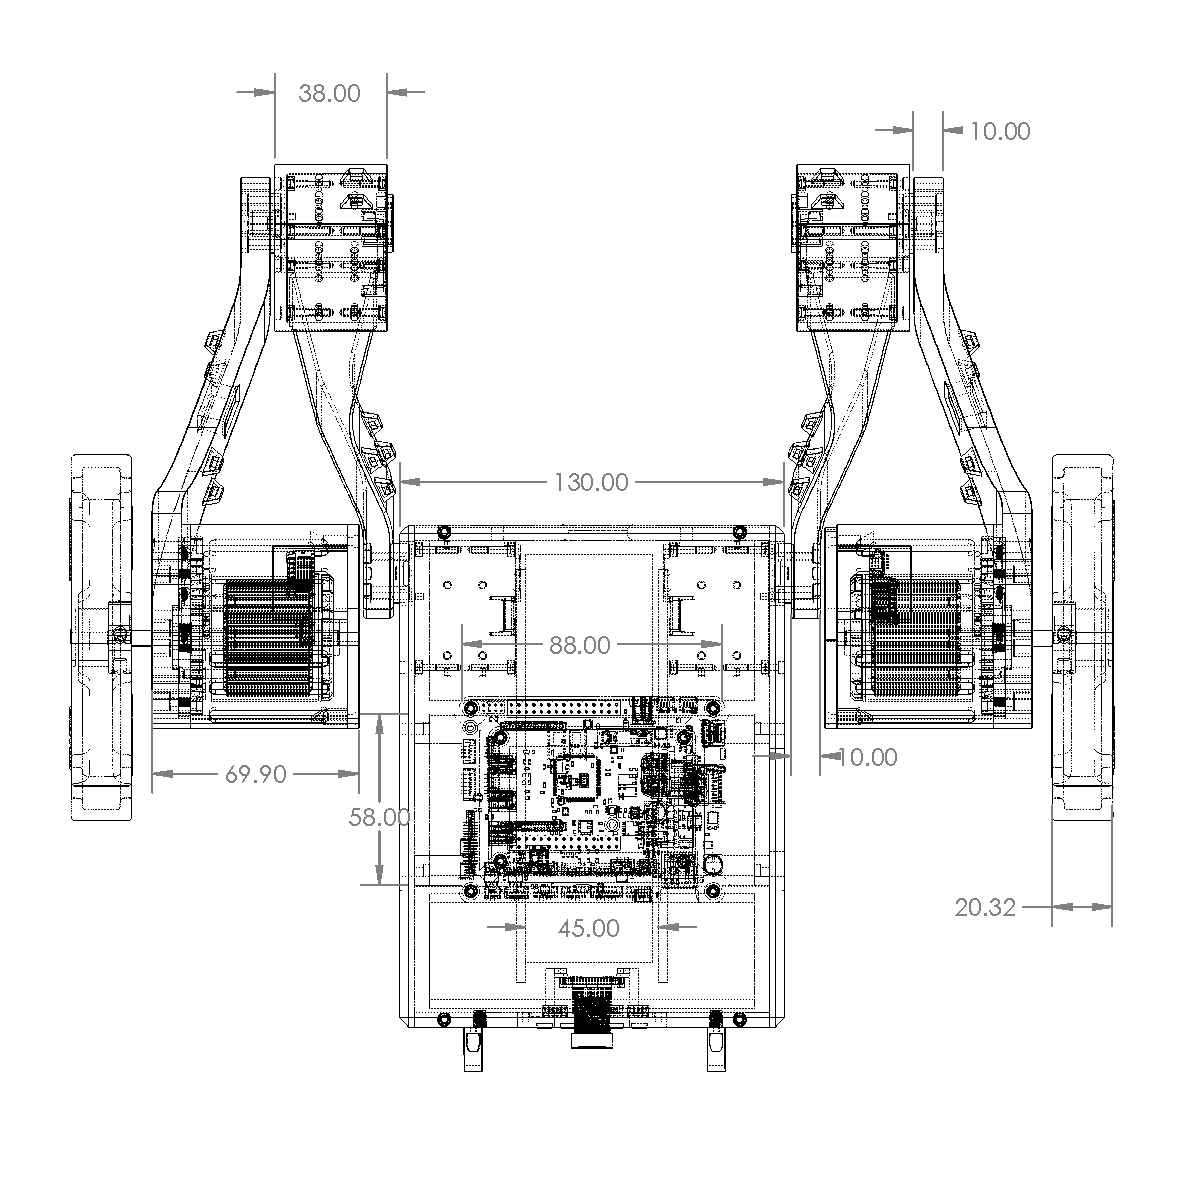
\includegraphics[width=\linewidth]{Robot_Assembly_V2_Top}
	\caption[Top view of the Robot Assembly]{Top view of the Robot Assembly}
	\label{fig:robotassemblyv2top}
\end{figure}

% three subfigures side by side of the robot assembly different configurations
\begin{figure}[h!]
	\centering
	\begin{subfigure}[b]{0.3\textwidth}
		\centering
		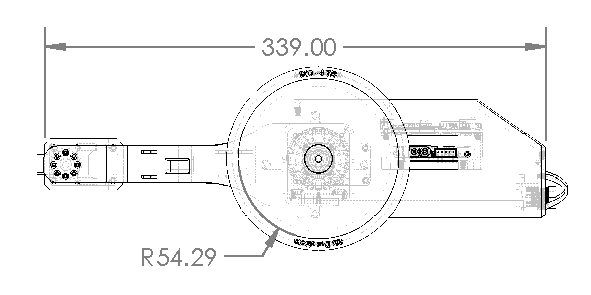
\includegraphics[width=.9\linewidth]{Robot_Assembly_V2_position_1}
		\caption{Robot Assembly Position 1}
		\label{fig:robotassemblyv2position1}
	\end{subfigure}
	\begin{subfigure}[b]{0.3\textwidth}
		\centering
		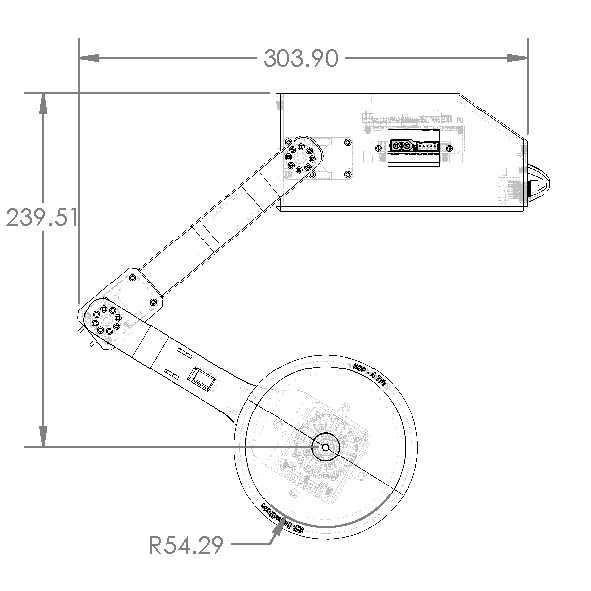
\includegraphics[width=.9\linewidth]{Robot_Assembly_V2_position_2}
		\caption{Robot Assembly Position 2}
		\label{fig:robotassemblyv2position2}
	\end{subfigure}
	\begin{subfigure}[b]{0.3\textwidth}
		\centering
		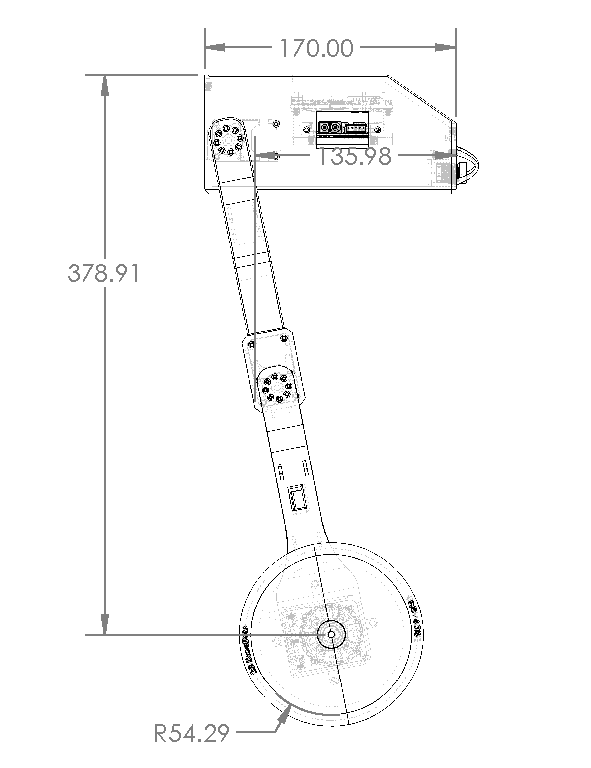
\includegraphics[width=.9\linewidth]{Robot_Assembly_V2_position_3}
		\caption{Robot Assembly Position 3}
		\label{fig:robotassemblyv2position3}
	\end{subfigure}
	\caption[Robot Assembly Different Configurations]{Robot Assembly Different Configurations}
	\label{fig:robotassemblyv2differentconfigurations}
\end{figure}

The figure above \ref{fig:robotassemblyv2differentconfigurations} shows the different configurations of the robot knee angle.
In position \ref{fig:robotassemblyv2position1}, the kip axis is aligned with the wheel axis, In position \ref{fig:robotassemblyv2position2}, the knee angle is changed to lift the body, In position \ref{fig:robotassemblyv2position3}, the hip angle is extended to its maximum angle.
Position \ref{fig:robotassemblyv2position2} and \ref{fig:robotassemblyv2position3} show that the robot's body will move a bit backwards by the control input to maintain the center of gravity of the robot above the wheel axis.


\subsection{Safety considerations}
% the motor cover, the face shield of the body and the body cover
Safety is a crucial aspect to consider in the design of the robot.
The robot is designed to be safe to operate in the environment and safe to interact with humans.
Clearances are considered in the design to make sure that moving parts wouldn't interfere with each other.
The motor cover is designed to protect the motor from any external objects that might interfere with the motor operation.
%Two subfigures side by side of the motor cover
%two subfigures side by side of the face shield
\begin{figure}[h]
	\centering
	\begin{subfigure}[b]{0.4\textwidth}
		\centering
		
\includegraphics[width=.5\linewidth]{Support_flexible_1}
		\caption{Face Shield Side View}
		\label{fig:face shield side view}
	\end{subfigure}
	\hfill
	\begin{subfigure}[b]{0.4\textwidth}
		\centering
		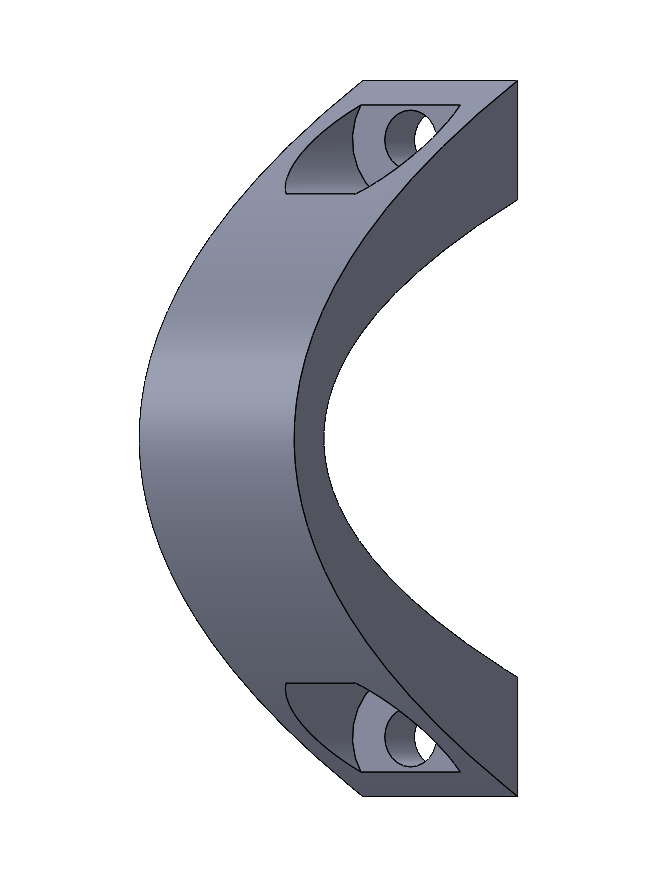
\includegraphics[width=.5\linewidth]{Support_flexible_2}
		\caption{Face Shield 3D View}
		\label{fig:faseshield3dview}
	\end{subfigure}
	\caption{Face Shield}
	\label{fig:faceshield}
\end{figure}

The face shield of the body is designed to protect the components inside the body.
The face shield is designed to be flexible to absorb the shock from any external objects that might hit the robot. It is screwed with two screws to the body.
%cable mangment
The cable management is considered in the design of the robot to make sure that the cables are routed from and to all the components in the robot in a safe way to protect the cables form tearing or getting damaged as well as to protect the cables from interfering with the movement of the robot.



\section{Design for Manufacturability and Assembly}
% Discuss how the design facilitates manufacturing and assembly.
% Explain any design choices made to simplify these processes of manufacturing and assembly.
% Discuss any design features that were added to facilitate the manufacturing and assembly processes.
Design for manufacturability and assembly was considered throughout the design process.
Design consideration was taken into account to make sure that the robot parts can be printed using 3D printing technology.
Considering the limitations of 3D printing technology, the design was modified to make sure that the parts can be printed with acceptable quality.
The orientation at which the parts are printed was considered while designing the parts.
Assembly fitting and clearance were considered to make sure that the parts can be assembled with ease.
\newpage
\section{Prototyping and Iterative Design}
% Discuss the process of prototyping.
% Explain how feedback from prototyping phases was incorporated into design revisions.

During the design process, the sketches for the different parts were drawn relying on each other so that future modifications can be easily applied.
 The design was prototyped using 3D printing.
Therefore, different problems were encountered during the prototyping process.
The problems were analyzed and the design was modified accordingly to solve the problems.
Some of the problems were related to the 3D printing process, and some were related to the design itself, such as the clearance between the parts, the cable management dimensions.
The actual physical parts were slightly different in dimensions than the CAD model.
This is why ititrations were made to the design.

